%  State of the art. 

% - add : Evaluate Collaboratory article 
% - add : the  hardware papers 


\subsection{docker and accuracy}
And now Since the stat of the art has aggreed on the impact of docker on the energy consumption,Let's discuss it's impact on the accuracy. In other words\\
\textbf{RQ :} does Docker affect the energy variation of the exepements ?

To Answer this question we have conducted a preliminary experiment by running the same benchmarks \textsf{LU}, \textsf{CG} and \textsf{EP} in a Docker container and a flat binary format on 3 nodes of the cluster \textsf{Dahu} to assess if Docker induces an additional variation.
Figure~\ref{fig:docker} reports that this is not the case, as the energy consumption variation does not get noticeably affected by Docker while running a same compiled version of the benchmarks at 5\,\%, 50\,\% and 100\,\% workloads.
In fact, while Docker increases the energy consumption due to the extra layer it implements~\cite{eddie_antonio_santos_how}, it does not noticeably affect the energy variation.
The \emph{standard deviation} (STD) is even slightly smaller ($STD_{Docker}=192 mJ$,$STD_{Binary}=207 mJ$), taking into account the measurements errors and the OS activity.

\begin{figure}
    \center{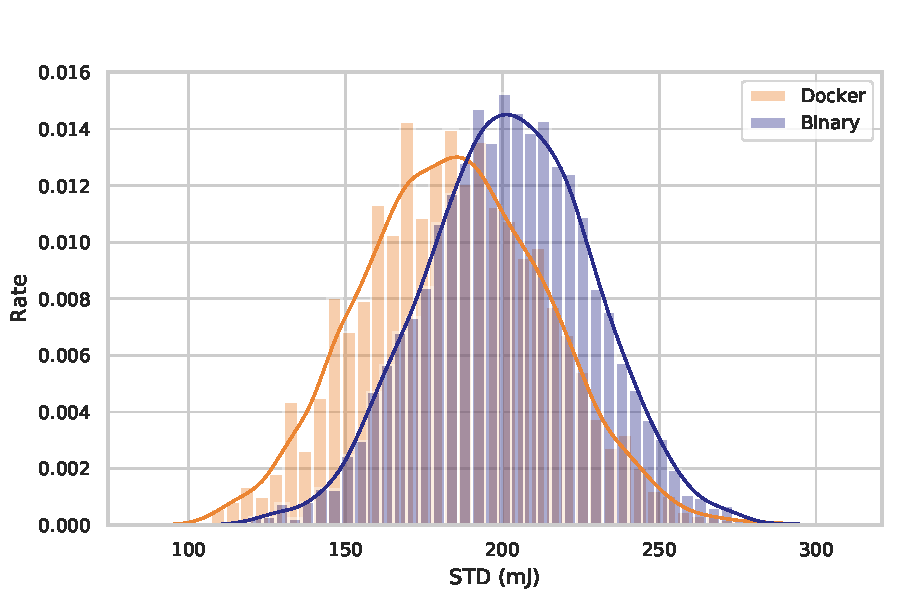
\includegraphics[width=.9\linewidth]{imgs/docvsbin}}
    \caption{Comparing the variation of binary and Docker versions of aggregated \textsf{LU}, \textsf{CG} and \textsf{EP} benchmarks}\label{fig:docker}
\end{figure}